\chapter{边界层理论}

\intro{边界层概念的提出是流体力学历史上最具洞察力的简化之一。Prandtl在1904年将NS方程分解为无粘外流与薄层粘性内流，解开了历时已久的D'Alembert佯谬。}

\section{边界层概念}

\subsection{Prandtl的洞察}

1904年，Ludwig Prandtl在海德堡国际数学家大会上首次提出了边界层（Grenzschicht）的概念，这彻底改变了流体力学的发展进程。

Prandtl观察到：对于高Reynolds数绕流，粘性效应仅限于壁面附近一薄层（边界层），而在边界层之外，流动可视作无粘势流。边界层厚度 $\delta$ 远小于流向特征长度 $L$（$\delta \ll L$），因此法向梯度远大于流向梯度（$\partial/\partial x \ll \partial/\partial y$）。

\subsection{壁面无滑移条件}

真实的粘性流体在固体壁面上相对于壁面的速度为零。这一条件与理想流体的滑移边界完全不同，是产生涡量和粘性阻力的根本原因。壁面无滑移导致：
\begin{itemize}
    \item 壁面处速度为零，远离壁面处速度渐恢复至外流速度
    \item 壁面法向存在极大的速度梯度，粘性切应力 $\tau_w = \mu\frac{\partial u}{\partial y}\big|_{y=0}$ 不可忽略
    \item 壁面是涡量的源泉：涡量在壁面产生并向流体内部扩散
\end{itemize}

\subsection{边界层厚度的定义}

\begin{mydefinition}{位移厚度}
边界层对外流施加的排移效应由位移厚度 $\delta^{*}$ 表征：
\begin{myformula}
    \delta^{*}(x) = \int_{0}^{\infty}\left(1 - \frac{u}{U_e}\right)dy
\end{myformula}
其中 $U_e(x)$ 为边界层外缘速度。
\end{mydefinition}

\begin{mydefinition}{动量厚度}
动量厚度 $\theta$ 与壁面摩擦阻力直接相关：
\begin{myformula}
    \theta(x) = \int_{0}^{\infty}\frac{u}{U_e}\left(1 - \frac{u}{U_e}\right)dy
\end{myformula}
\end{mydefinition}

常见的名义厚度 $\delta_{99}$ 定义为 $u=0.99U_e$ 处距壁面的法向距离。

\begin{figure}[H]
\centering
\begin{tikzpicture}[scale=1.3]
    \definecolor{myBLcol}{RGB}{180,210,250}
    \definecolor{myWallcol}{RGB}{60,60,60}
    \definecolor{myProfcol}{RGB}{20,60,150}
    \definecolor{myOuter}{RGB}{200,100,30}
    
    \fill[myWallcol] (0,-0.2) rectangle (8,0);
    \draw[->, line width=1.5pt] (0,0) -- (8,0) node[right] {$x$};
    \draw[->, line width=1.5pt] (0,0) -- (0,4) node[above] {$y$};
    
    \fill[myBLcol!40] (0,0) to[out=30, in=210] (8,2.5) -- (8,0) -- cycle;
    \draw[dashed] (0,0) to[out=30, in=210] (8,2.5);
    \node at (7.8,2.8) {$\delta(x)$};
    
    \draw[myOuter, line width=1.8pt] (0,3.2) -- (8,3.2);
    \node[myOuter] at (4,3.5) {外流 $U_e$};
    
    \draw[myProfcol, line width=2pt, domain=0.02:3, samples=50, variable=\y]
        plot ({3+(3.0-\y)/(2.5*\y)}, {\y});
    \draw[myProfcol, line width=2pt, domain=0.02:3.5, samples=50, variable=\y]
        plot ({6+(3.5-\y)/(2.5*\y)}, {\y});
    
    \node at (5,1.0) {边界层};
    \node at (3.2,-0.4) {层流};
    \node at (6.5,-0.4) {湍流};
\end{tikzpicture}
\caption{边界层发展示意：壁面上边界层增长及层流向湍流的转捩}
\label{fig:bl-development}
\end{figure}

\section{边界层方程的推导}

\subsection{量纲分析与NS方程的简化}

从二维定常不可压缩NS方程出发。设定特征尺度：$x \sim L$，$y \sim \delta$，$u \sim U$，$v \sim U\delta/L$。代入连续性方程和动量方程：

\begin{itemize}
    \item 连续性：$\frac{\partial u}{\partial x} \sim \frac{U}{L}$，$\frac{\partial v}{\partial y} \sim \frac{U}{L}$，两项同量纲
    \item $x$ 方向动量粘性项：$\nu\frac{\partial^{2}u}{\partial x^{2}} \sim \frac{\nu U}{L^{2}}$，$\nu\frac{\partial^{2}u}{\partial y^{2}} \sim \frac{\nu U}{\delta^{2}}$
    \item $\delta \ll L$ 故可忽略流向扩散
    \item $y$ 方向动量退化为 $\frac{\partial p}{\partial y} \approx 0$，压力在边界层法向为常数
\end{itemize}

\subsection{二维定常Prandtl边界层方程}

经简化得到经典的边界层方程：

\begin{myformula}
    u\frac{\partial u}{\partial x} + v\frac{\partial u}{\partial y} = U_e\frac{dU_e}{dx} + \nu\frac{\partial^{2} u}{\partial y^{2}}
\end{myformula}

配合连续性方程 $\frac{\partial u}{\partial x} + \frac{\partial v}{\partial y} = 0$ 和边界条件：

\begin{myformula}
    y=0:\; u=v=0 \quad\text{（无滑移边界）};\qquad
    y\to\infty:\; u \to U_e(x) \quad\text{（外部势流匹配）}
\end{myformula}

其中压力梯度项 $U_e\frac{dU_e}{dx}$ 通过与外部无粘势流耦合由Bernoulli方程 $p(x) + \frac{1}{2}\rho U_e^{2}(x) = \mathrm{const}$ 确定。

\begin{remark}
Prandtl边界层方程是抛物型的（$x$ 方向为演化方向），而原始NS方程是椭圆型的。这一降阶简化极大地降低了数学难度，但丧失了流向信息的上游传播能力。
\end{remark}

\section{Blasius解}

\subsection{相似变换}

Blasius（1908年）求解了零压力梯度（$dU_e/dx=0$）平板边界层的自相似解。引入流函数 $\psi$（$u=\partial\psi/\partial y$，$v=-\partial\psi/\partial x$）和相似变量：

\begin{myformula}
    \eta = y\sqrt{\frac{U_{\infty}}{\nu x}},\qquad
    f(\eta) = \frac{\psi}{\sqrt{\nu x U_{\infty}}}
\end{myformula}

边界层PDE化为关于 $f(\eta)$ 的Blasius三阶ODE：

\begin{myformula}
    2f''' + ff'' = 0
\end{myformula}

边界条件：$f(0)=f'(0)=0$（无滑移），$f'(\infty)=1$（匹配外流）。

\subsection{数值求解（打靶法）}

Blasius方程是三阶非线性两点边值问题。采用打靶法求解：猜测壁面值 $f''(0)$，从壁面向前积分到无穷远，迭代至 $f'(\infty) \to 1$。标准结果：$f''(0) \approx 0.332057$。

\begin{mycode}{Python：Blasius方程的打靶法求解}
\begin{lstlisting}[language=Python]
import numpy as np
from scipy.integrate import solve_ivp
from scipy.optimize import root_scalar

def blasius_ode(eta, y):
    f, fp, fpp = y
    return [fp, fpp, -0.5 * f * fpp]

def solve_blasius(shoot_guess, eta_max=10.0):
    sol = solve_ivp(blasius_ode, [0, eta_max],
        [0.0, 0.0, shoot_guess],
        t_eval=np.linspace(0, eta_max, 500),
        method='RK45', rtol=1e-10, atol=1e-12)
    return sol

def shoot_error(fpp0):
    sol = solve_blasius(fpp0, eta_max=15.0)
    return sol.y[1, -1] - 1.0

result = root_scalar(shoot_error, bracket=[0.1, 0.5],
    method='bisection', xtol=1e-10)
fpp0 = result.root

sol = solve_blasius(fpp0, eta_max=10.0)
print(f"f''(0) = {fpp0:.8f}")
print(f"Verified: f'(inf) = {sol.y[1,-1]:.8f}")

delta_99 = sol.t[np.argmin(np.abs(sol.y[1,:] - 0.99))]
delta_star = np.trapz(1 - sol.y[1,:], sol.t)
theta = np.trapz(sol.y[1,:] * (1 - sol.y[1,:]), sol.t)

print(f"delta_99 / sqrt(nu*x/U) = {delta_99:.4f}")
print(f"delta*  / sqrt(nu*x/U) = {delta_star:.4f}")
print(f"theta  / sqrt(nu*x/U) = {theta:.4f}")
\end{lstlisting}
\end{mycode}

\subsection{Blasius解的主要结果}

\begin{itemize}
    \item 壁面摩擦系数 $c_f = \frac{\tau_w}{\frac{1}{2}\rho U_{\infty}^{2}} = \frac{0.664}{\sqrt{Re_x}}$
    \item 名义厚度 $\delta_{99} = \frac{5.0 x}{\sqrt{Re_x}}$，位移厚度 $\delta^{*} \approx \frac{1.7208 x}{\sqrt{Re_x}}$
    \item 动量厚度 $\theta \approx \frac{0.664 x}{\sqrt{Re_x}}$，形状因子 $H = \delta^{*}/\theta \approx 2.59$
\end{itemize}

\begin{figure}[H]
\centering
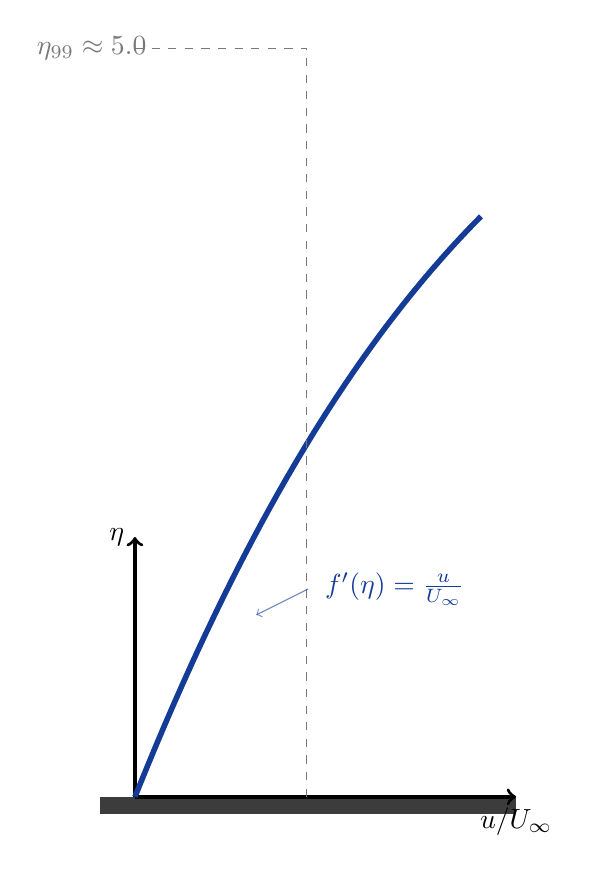
\begin{tikzpicture}[scale=2.2]
    \definecolor{mycur}{RGB}{20,60,150}
    \definecolor{mywal}{RGB}{60,60,60}
    \definecolor{myref}{RGB}{120,120,120}
    
    \fill[mywal] (-0.2,-0.1) rectangle (2.2,0);
    \draw[->, line width=1.2pt] (0,0) -- (2.2,0) node[below] {$u/U_{\infty}$};
    \draw[->, line width=1.2pt] (0,0) -- (0,1.5) node[left] {$\eta$};
    
    \draw[mycur, line width=2pt, domain=0:2, samples=200, smooth, variable=\x]
        plot ({\x}, {5.0 * (1 - exp(-0.5*\x* (1+0.332*\x/6)))});
    
    \draw[myref, dashed] (0.99,0) -- (0.99,5*0.864);
    \draw[myref, dashed] (0,5*0.864) -- (0.99,5*0.864);
    \node[myref] at (-0.25, 5*0.864) {$\eta_{99}\approx 5.0$};
    
    \node[mycur] at (1.5, 1.2) {$f'(\eta)=\frac{u}{U_{\infty}}$};
    \draw[->, mycur, opacity=0.6] (1.0, 1.2) -- (0.7, 1.05);
\end{tikzpicture}
\caption{Blasius速度剖面 $f'(\eta)=u/U_{\infty}$，$\eta_{99}\approx 5.0$ 对应 $u=0.99U_{\infty}$}
\label{fig:blasius-profile}
\end{figure}

\section{边界层的积分方法}

\subsection{Von Karman动量积分方程}

对边界层方程从壁面积分到无穷远，得到von Karman动量积分方程：

\begin{myformula}
    \frac{\tau_w}{\rho} = \frac{d}{dx}(U_e^{2}\theta) + \delta^{*} U_e\frac{dU_e}{dx}
\end{myformula}

或等价形式：

\begin{myformula}
    \frac{d\theta}{dx} + (2+H)\frac{\theta}{U_e}\frac{dU_e}{dx} = \frac{c_f}{2}
\end{myformula}

其中 $H = \delta^{*}/\theta$ 为形状因子，$c_f = \tau_w/(\frac{1}{2}\rho U_e^{2})$。

\subsection{Pohlhausen方法}

Pohlhausen（1921年）假设速度剖面用四次多项式表示：

\begin{myformula}
    \frac{u}{U_e} = F(\eta) + \Lambda G(\eta),\quad \eta = \frac{y}{\delta(x)}
\end{myformula}

其中 $\Lambda = \frac{\delta^{2}}{\nu}\frac{dU_e}{dx}$ 为无量纲压力梯度参数。$\Lambda > 0$ 对应顺压力梯度（加速流），$\Lambda < 0$ 对应逆压力梯度（减速流）。分离判据为 $\Lambda \approx -12$。

\subsection{Thwaites方法}

Thwaites（1949年）通过对大量精确解数据拟合，提出了无需迭代的动量厚度公式：

\begin{myformula}
    \theta^{2} = \frac{0.45\nu}{U_e^{6}}\int_{0}^{x} U_e^{5}(s)\,ds
\end{myformula}

该公式简单而精确，是工程快速估算层流边界层的优秀工具。

\begin{example}
对 $U_e(x)=U_0(1-x/L)$ 的线性减速流（逆压力梯度），应用Thwaites公式得分离点位于 $x/L \approx 0.12$。
\end{example}

\section{边界层分离}

\subsection{分离的物理机制}

当流体遇到逆压力梯度（$dp/dx > 0$，即 $dU_e/dx < 0$），壁面附近的低动量流体难以克服不断增大的压力，速度渐减至零乃至反向。流线被迫离开壁面，形成分离区。分离的数学条件是：

\begin{myformula}
    \tau_w = \mu\frac{\partial u}{\partial y}\bigg|_{y=0} = 0
\end{myformula}

边界层分离导致压差阻力大幅增加、升力降低，以及可能的涡脱落与非定常载荷。

\subsection{分离的控制}

通过适当方法可推迟或抑制分离：
\begin{itemize}
    \item 顺压力梯度（加速流）推迟分离
    \item 边界层吹吸：吹气增加低速区动量，吸气移除低动量流体
    \item 涡流发生器诱导流向涡，将高动量外流带入近壁区
    \item 湍流边界层混合能力强，比层流更抗分离
\end{itemize}

\subsection{尾迹区}

分离后形成尾迹（wake），其宽度和动量亏损决定压差阻力。钝体（圆柱、球）分离较早，压差阻力主导；流线体（翼型）分离延迟至后缘，摩擦阻力主导。远尾迹自相似解中心线速度亏损以 $x^{-1/2}$ 衰减。

\section{层流边界层的转捩}

\subsection{转捩的工程意义}

边界层从层流转换为湍流时，摩擦系数、传热率和分离特性均显著变化。湍流边界层壁面摩擦约为层流的5-10倍（同一Re下），故准确预测转捩位置对阻力估算至关重要。

\subsection{影响转捩的因素}

\begin{itemize}
    \item Reynolds数：$Re$ 越高越易转捩，基于动量厚度的 $Re_{\theta,tr}$ 是常用判据
    \item 压力梯度：顺压力梯度（加速）稳定层流推迟转捩；逆压力梯度（减速）促进转捩
    \item 来流湍流度：高湍流度显著降低临界Re
    \item 壁面粗糙度：诱发局部扰动，降低转捩Re
    \item 壁面曲率：凹壁面Gortler涡促进转捩
\end{itemize}

\subsection{自然转捩与旁路转捩}

\textbf{自然转捩}（低来流湍流度）：遵循T-S波线性增长、非线性饱和、二次失稳、湍斑形成、充分湍流的标准路径。\textbf{旁路转捩}（中高来流湍流度）：来流扰动直接激发近壁条带结构和Klebanoff模，绕过T-S波阶段直接湍斑形成，在叶轮机械内流中非常常见。

\section{湍流边界层}

\subsection{湍流边界层的多层结构}

从壁面向外依次为：

\begin{itemize}
    \item \textbf{粘性底层}（$y^{+} < 5$）：分子粘性主导，$u^{+} = y^{+}$
    \item \textbf{过渡层/缓冲层}（$5 < y^{+} < 30$）：粘性应力与湍流应力同等重要，湍动能产生率最大
    \item \textbf{对数区}（$y^{+} > 30$，$y/\delta < 0.2$）：湍流主导，服从对数律
    \item \textbf{外层/尾迹区}（$y/\delta > 0.2$）：偏离对数律，需尾迹函数修正
\end{itemize}

其中 $y^{+} = y u_{\tau}/\nu$，$u_{\tau} = \sqrt{\tau_w/\rho}$ 为摩擦速度，$u^{+} = u/u_{\tau}$。

\subsection{壁面律（Law of the Wall）}

对数区的经典表达式（光滑壁面）：

\begin{myformula}
    u^{+} = \frac{1}{\kappa}\ln y^{+} + B
\end{myformula}

其中 $\kappa \approx 0.41$ 为von Karman常数，$B \approx 5.0$。考虑尾迹效应的完整剖面（Coles尾迹律）：

\begin{myformula}
    u^{+} = \frac{1}{\kappa}\ln y^{+} + B + \frac{2\Pi}{\kappa}W\left(\frac{y}{\delta}\right)
\end{myformula}

$\Pi \approx 0.55$ 为尾迹强度参数，$W(\eta) = 2\sin^{2}(\pi\eta/2)$ 为尾迹函数。

\begin{figure}[H]
\centering
\begin{tikzpicture}[scale=1.6]
    \definecolor{mycurvel}{RGB}{20,60,150}
    \definecolor{myvisc}{RGB}{180,40,40}
    \definecolor{mylog}{RGB}{40,120,40}
    \definecolor{myreg}{RGB}{100,100,100}
    
    \draw[->, line width=1.2pt] (0,0) -- (6.5,0) node[below] {$\ln y^{+}$};
    \draw[->, line width=1.2pt] (0,0) -- (0,5.5) node[left] {$u^{+}$};
    
    \draw[myvisc, line width=2pt, domain=0:1.6, samples=50, variable=\x]
        plot ({\x}, {exp(\x)});
    \node[myvisc] at (0.3, 3.2) {$u^{+}=y^{+}$};
    
    \pgfmathsetmacro{\kp}{0.41}
    \pgfmathsetmacro{\Bval}{5.0}
    \draw[mylog, line width=2pt, domain=1.3:5.8, samples=50, variable=\x]
        plot ({\x}, {\x/\kp + \Bval - 3.0});
    \node[mylog] at (5.2, 3.8) {$\frac{1}{\kappa}\ln y^{+}+B$};
    
    \draw[mycurvel, line width=2.5pt, domain=0:6, samples=200, variable=\x]
        plot ({\x}, {min(exp(\x), \x/\kp + \Bval - 3.0
            + 0.5*sin(180*min(1,(\x-2.5)/3.5)^2*pi/180 r))});
    
    \draw[myreg, dashed] (1.6, 0.1) -- (1.6, 5.0);
    \draw[myreg, dashed] (3.4, 0.1) -- (3.4, 5.0);
    \node[myreg] at (0.7, 1.0) {粘性底层};
    \node[myreg] at (2.4, 1.6) {过渡层};
    \node[myreg] at (4.5, 2.5) {对数区};
    \node[myreg] at (5.3, 4.6) {尾迹区};
\end{tikzpicture}
\caption{湍流边界层壁面律：粘性底层、对数区和尾迹区（半对数坐标）}
\label{fig:law-of-wall}
\end{figure}

\subsection{湍流边界层的统计特性}

$u'_{\mathrm{rms}}$ 在 $y^{+} \approx 15$ 附近达到最大值（$u'_{\mathrm{rms}}/u_{\tau} \approx 2.7$）。$v'_{\mathrm{rms}}$ 受壁面强烈抑制，最大值在 $y^{+} \approx 50-100$ 处。Reynolds剪切应力 $-\overline{u'v'}$ 在内层（$y/\delta < 0.3$）近似为常数 $u_{\tau}^{2}$。

典型的湍流结构包括：近壁高低速条带结构（间距约 $100\nu/u_{\tau}$）、猝发事件（低速条带上扬、高速流体下扫）以及外层大尺度运动对近壁湍流的调制。

\subsection{平板湍流边界层的摩擦阻力}

1/7次方速度剖面近似给出的局部和总摩擦系数：

\begin{myformula}
    c_f = \frac{0.027}{Re_x^{1/7}},\qquad
    C_F = \frac{0.031}{Re_L^{1/7}}
\end{myformula}

更精确的Prandtl-Schlichting对数律：

\begin{myformula}
    c_f = [2\log_{10}(Re_x) - 0.65]^{-2.3}
\end{myformula}

湍流边界层的摩擦阻力显著大于层流。$Re_L = 10^{6}$ 时全湍流平板摩擦阻力系数约为全层流平板的3倍以上。

\subsection{粗糙度对湍流边界层的影响}

等效砂粒粗糙度 $k_s$，粗糙度Reynolds数 $k_s^{+} = k_s u_{\tau}/\nu$：
\begin{itemize}
    \item 水力光滑（$k_s^{+} < 5$）：粗糙度浸没于粘性底层，无影响
    \item 过渡粗糙（$5 < k_s^{+} < 70$）：对数律截距减小
    \item 完全粗糙（$k_s^{+} > 70$）：摩擦系数与Re无关，壁面律修正为 $u^{+} = \frac{1}{\kappa}\ln(y/k_s) + 8.5$
\end{itemize}

\begin{mycode}{Python：平板边界层摩擦系数计算}
\begin{lstlisting}[language=Python]
import numpy as np
import matplotlib.pyplot as plt

def blasius_friction(Re_x):
    return 0.664 / np.sqrt(Re_x)

def turbulent_friction_17(Re_x):
    return 0.027 / Re_x**(1/7)

def turbulent_friction_log(Re_x):
    return (2*np.log10(Re_x) - 0.65)**(-2.3)

Re_x = np.logspace(4, 8, 200)
c_f_lam = blasius_friction(Re_x)
c_f_turb17 = turbulent_friction_17(Re_x)
c_f_turb_log = turbulent_friction_log(Re_x)

fig, ax = plt.subplots(figsize=(8, 5))
ax.loglog(Re_x, c_f_lam, 'b-', linewidth=2,
    label='Laminar (Blasius)')
ax.loglog(Re_x, c_f_turb17, 'r--', linewidth=2,
    label='Turbulent (1/7 power)')
ax.loglog(Re_x, c_f_turb_log, 'g-.', linewidth=2,
    label='Turbulent (Log-law)')
ax.axvline(5e5, color='gray', linestyle=':')
ax.text(5.2e5, 0.01, '$Re_{cr}$', fontsize=11)
ax.set_xlabel('$Re_x$'); ax.set_ylabel('$c_f$')
ax.legend(); ax.grid(True, alpha=0.3)
ax.set_ylim([5e-4, 2e-2])
plt.tight_layout(); plt.show()

Re_tr = 5e5; Re_L = 1e7
theta_tr = 0.664 * Re_tr**(-0.5)
C_F_mixed = (0.074*Re_L**(-1/5) - 0.074*Re_tr**(-1/5)
    + theta_tr * Re_tr/Re_L)
C_F_turb = 0.074 * Re_L**(-1/5)
C_F_lam = 1.328 * Re_L**(-0.5)
print(f"Laminar C_F = {C_F_lam:.4f}")
print(f"Turbulent C_F = {C_F_turb:.4f}")
print(f"Mixed BL C_F = {C_F_mixed:.4f}")
\end{lstlisting}
\end{mycode}

\section{三维边界层}

当外部势流具有横向速度分量（如后掠翼、旋转体）时，边界层是三维的。三维边界层的主要特征是存在横向流动（cross-flow）和极限流线（limiting streamline）。

壁面剪切应力方向定义了极限流线方向：$\frac{dz}{dx}\big|_{y=0} = \frac{\tau_{w,z}}{\tau_{w,x}}$。三维边界层的分离不简单地由壁面切应力为零判定，而是由极限流线的拓扑奇点（鞍点、结点、螺旋点）决定。

旋转圆盘上的边界层是三维边界层的经典问题（von Karman, 1921）。由于离心力，近壁流体向外甩出，轴向流体向盘面补充。通过相似变换，问题化为关于无量纲速度剖面 $F(\eta)$、$G(\eta)$ 和 $H(\eta)$ 的耦合ODE系统，其中 $\eta = z\sqrt{\omega/\nu}$。

\section{本章总结}

本章从Prandtl边界层概念出发，系统阐述了边界层理论的数学基础。通过量纲分析导出了Prandtl边界层方程，获得了零压力梯度下的Blasius精确自相似解。积分方法（von Karman动量积分、Pohlhausen方法、Thwaites方法）为工程边界层计算提供了实用工具。边界层分离是决定绕流物体阻力的关键物理现象。湍流边界层的多层结构与壁面律构成了壁面湍流的理论框架，而三维边界层扩展了理论在航空航天等领域的应用范围。
